% questions.tex —— 2013 年·辽宁卷·文科 · 题目内容片段（无答案）
% 由 tools/generate_projects.py 依来源总账自 2013/2013_数学真题_辽宁文_试题.md 生成，勿手改（改源 MD 后重跑）

\gkpart{一、选择题}

\begin{question}
\gkti{1}已知集合 $A=\{0,1,2,3,4\}$，$B=\{x\mid |x|<2\}$，则 $A\cap B=$\mbox{（　　）}

（A）$\{0\}$；（B）$\{0,1\}$；（C）$\{0,2\}$；（D）$\{0,1,2\}$。

\end{question}
\begin{question}
\gkti{2}复数 $z=\dfrac{1}{\mathrm i-1}$ 的模为\mbox{（　　）}

（A）$\dfrac12$；（B）$\dfrac{\sqrt2}2$；（C）$\sqrt2$；（D）$2$。

\end{question}
\begin{question}
\gkti{3}已知点 $A(1,3)$，$B(4,-1)$，则与向量 $\overrightarrow{AB}$ 同方向的单位向量为\mbox{（　　）}

（A）$\left(\dfrac35,-\dfrac45\right)$；（B）$\left(\dfrac45,-\dfrac35\right)$；（C）$\left(-\dfrac35,\dfrac45\right)$；（D）$\left(-\dfrac45,\dfrac35\right)$。

\end{question}
\begin{question}
\gkti{4}下面是关于公差 $d>0$ 的等差数列 $\{a_n\}$ 的四个命题：

$p_1$：数列 $\{a_n\}$ 是递增数列；

$p_2$：数列 $\{na_n\}$ 是递增数列；

$p_3$：数列 $\left\{\dfrac{a_n}{n}\right\}$ 是递增数列；

$p_4$：数列 $\{a_n+3nd\}$ 是递增数列。

其中的真命题为\mbox{（　　）}

（A）$p_1$，$p_2$；（B）$p_3$，$p_4$；（C）$p_2$，$p_3$；（D）$p_1$，$p_4$。

\Needspace{0.4\textheight}
\end{question}
\begin{question}
\gkti{5}某班的全体学生参加英语测试，成绩的频率分布直方图如图，数据的分组依次为：$[20,40)$，$[40,60)$，$[60,80)$，$[80,100]$。若低于 $60$ 分的人数是 $15$，则该班的学生人数是\mbox{（　　）}
\nopagebreak[4]
\begin{center}% 2013 辽宁卷文科第 5 题：成绩频率分布直方图。
\begin{tikzpicture}[font=\footnotesize, >=Stealth, line width=0.5pt,
  x=1.15cm, y=160cm]
  % 坐标轴：横轴以 20 分为一个单位
  \draw[->] (0,0) -- (5.75,0) node[right, yshift=-2pt] {成绩/分};
  \draw[->] (0,0) -- (0,0.0238);
  \node at (0,0.0295) {$\dfrac{\text{频率}}{\text{组距}}$};
  % 横轴刻度
  \foreach \x/\lab in {0/0,1/20,2/40,3/60,4/80,5/100}
    \draw (\x,0) -- (\x,-0.0006) node[below] {$\lab$};
  % 纵轴刻度与虚线
  \foreach \y/\lab in {0.005/0.005,0.010/0.010,0.015/0.015,0.020/0.020} {
    \draw (0,\y) -- (-0.08,\y) node[left] {$\lab$};
    \draw[dashed] (0,\y) -- (5.05,\y);
  }
  % 四个矩形：高度依次为 0.005、0.010、0.020、0.015
  \foreach \i/\h in {1/0.005,2/0.010,3/0.020,4/0.015} {
    \draw[fill=white] (\i-1,0) rectangle (\i,\h);
  }
\end{tikzpicture}
\end{center}
\nopagebreak[4]
（A）$45$；（B）$50$；（C）$55$；（D）$60$。

\end{question}
\begin{question}
\gkti{6}在 $\triangle ABC$ 中，内角 $A$，$B$，$C$ 所对的边分别为 $a$，$b$，$c$，若 $a\sin B\cos C+c\sin B\cos A=\dfrac12b$，且 $a>b$，则 $\angle B=$\mbox{（　　）}

（A）$\dfrac\pi6$；（B）$\dfrac\pi3$；（C）$\dfrac{2\pi}3$；（D）$\dfrac{5\pi}6$。

\end{question}
\begin{question}
\gkti{7}已知函数 $f(x)=\ln\left(\sqrt{1+9x^2}-3x\right)+1$，则 $f(\lg 2)+f\left(\lg\dfrac12\right)=$\mbox{（　　）}

（A）$-1$；（B）$0$；（C）$1$；（D）$2$。

\Needspace{0.4\textheight}
\end{question}
\begin{question}
\gkti{8}执行如图所示的程序框图，若输入 $n=8$，则输出 $S=$\mbox{（　　）}
\nopagebreak[4]
\begin{center}% 2013 辽宁卷文科第 8 题：程序框图。
\begin{tikzpicture}[font=\footnotesize, >=Stealth, line width=0.45pt,
  node distance=5mm,
  term/.style={draw, rounded corners=6pt, minimum height=1.8em, inner xsep=9pt},
  io/.style={draw, trapezium, trapezium left angle=70, trapezium right angle=110,
             minimum height=1.8em, inner xsep=6pt},
  box/.style={draw, minimum height=1.9em, inner xsep=6pt},
  dec/.style={draw, diamond, aspect=2.2, inner sep=1pt}]
  \node[term] (start) {开始};
  \node[io, below=5mm of start] (input) {输入 $n$};
  \node[box, below=5mm of input] (init) {$S=0$，$i=2$};
  \node[dec, below=6mm of init] (cond) {$i\leqslant n$};
  \node[box, below=7mm of cond] (acc) {$S=S+\dfrac{1}{i^2-1}$};
  \node[box, below=5mm of acc] (inc) {$i=i+2$};
  \node[io, right=15mm of cond] (output) {输出 $S$};
  \node[term, below=6mm of output] (end) {结束};
  \draw[->] (start) -- (input);
  \draw[->] (input) -- (init);
  \draw[->] (init) -- (cond);
  \draw[->] (cond) -- node[right] {是} (acc);
  \draw[->] (acc) -- (inc);
  \draw[->] (cond) -- node[above] {否} (output);
  \draw[->] (output) -- (end);
  % 循环支路：从 i=i+2 左侧引出，向上回到判断框入口
  \draw[->] (inc.west) -- ++(-1.45,0) |- (cond.west);
\end{tikzpicture}
\end{center}
\nopagebreak[4]
（A）$\dfrac49$；（B）$\dfrac67$；（C）$\dfrac89$；（D）$\dfrac{10}{11}$。

\end{question}
\begin{question}
\gkti{9}已知点 $O(0,0)$，$A(0,b)$，$B(a,a^3)$。若 $\triangle OAB$ 为直角三角形，则必有\mbox{（　　）}

（A）$b=a^3$；（B）$b=a^3+\dfrac1a$；（C）$(b-a^3)\left(b-a^3-\dfrac1a\right)=0$；（D）$\left|b-a^3\right|+\left|b-a^3-\dfrac1a\right|=0$。

\end{question}
\begin{question}
\gkti{10}已知直三棱柱 $ABC-A_1B_1C_1$ 的 $6$ 个顶点都在球 $O$ 的球面上。若 $AB=3$，$AC=4$，$AB\perp AC$，$AA_1=12$，则球 $O$ 的半径为\mbox{（　　）}

（A）$\dfrac{3\sqrt{17}}2$；（B）$2\sqrt{10}$；（C）$\dfrac{13}2$；（D）$3\sqrt{10}$。

\end{question}
\begin{question}
\gkti{11}已知椭圆 $C:\dfrac{x^2}{a^2}+\dfrac{y^2}{b^2}=1\ (a>b>0)$ 的左焦点为 $F$，$C$ 与过原点的直线相交于 $A$，$B$ 两点，连接 $AF$，$BF$。若 $|AB|=10$，$|BF|=8$，$\cos\angle ABF=\dfrac45$，则 $C$ 的离心率为\mbox{（　　）}

（A）$\dfrac35$；（B）$\dfrac57$；（C）$\dfrac45$；（D）$\dfrac67$。

\end{question}
\begin{question}
\gkti{12}已知函数 $f(x)=x^2-2(a+2)x+a^2$，$g(x)=-x^2+2(a-2)x-a^2+8$，设 $H_1(x)=\max\{f(x),g(x)\}$，$H_2(x)=\min\{f(x),g(x)\}$（$\max\{p,q\}$ 表示 $p$，$q$ 中的较大值，$\min\{p,q\}$ 表示 $p$，$q$ 中的较小值）。记 $H_1(x)$ 的最小值为 $A$，$H_2(x)$ 的最大值为 $B$，则 $A-B=$\mbox{（　　）}

（A）$16$；（B）$-16$；（C）$a^2-2a-16$；（D）$a^2+2a-16$。

\end{question}
\gkpart{二、填空题}

\Needspace{0.4\textheight}
\begin{question}
\gkti{13}某几何体的三视图如图所示，则该几何体的体积是\gkblank{}。
\nopagebreak[4]
\begin{center}% 2013 辽宁卷文科第 13 题：某几何体的三视图。
\begin{tikzpicture}[font=\footnotesize, line width=0.5pt, >=Stealth]
  % 正视图：宽 4、高 4 的矩形，内部两条虚线分出其宽为 1、2、1
  \begin{scope}[shift={(0,0)}]
    \draw (0,0) rectangle (4,4);
    \draw[dashed] (1,0) -- (1,4);
    \draw[dashed] (3,0) -- (3,4);
    % 上方尺寸标注
    \draw[<->] (0,4.45) -- (1,4.45) node[midway, above] {$1$};
    \draw[<->] (1,4.45) -- (3,4.45) node[midway, above] {$2$};
    \draw[<->] (3,4.45) -- (4,4.45) node[midway, above] {$1$};
    \draw (0,4) -- (0,4.6);
    \draw (1,4) -- (1,4.6);
    \draw (3,4) -- (3,4.6);
    \draw (4,4) -- (4,4.6);
    % 左侧高度标注
    \draw[<->] (-0.45,0) -- (-0.45,4) node[midway, left] {$4$};
    \draw (0,0) -- (-0.6,0);
    \draw (0,4) -- (-0.6,4);
  \end{scope}
  % 侧视图
  \begin{scope}[shift={(5.6,0)}]
    \draw (0,0) rectangle (4,4);
    \draw[dashed] (1,0) -- (1,4);
    \draw[dashed] (3,0) -- (3,4);
    \draw[<->] (0,4.45) -- (1,4.45) node[midway, above] {$1$};
    \draw[<->] (1,4.45) -- (3,4.45) node[midway, above] {$2$};
    \draw[<->] (3,4.45) -- (4,4.45) node[midway, above] {$1$};
    \draw (0,4) -- (0,4.6);
    \draw (1,4) -- (1,4.6);
    \draw (3,4) -- (3,4.6);
    \draw (4,4) -- (4,4.6);
  \end{scope}
  % 俯视图：圆内接一个边长为 2 的正方形
  \begin{scope}[shift={(2.8,-4.9)}]
    \draw (0,0) circle (2);
    \draw (-1,-1) rectangle (1,1);
  \end{scope}
\end{tikzpicture}
\end{center}
\nopagebreak[4]
\end{question}
\begin{question}
\gkti{14}已知等比数列 $\{a_n\}$ 是递增数列，$S_n$ 是 $\{a_n\}$ 的前 $n$ 项和，若 $a_1$，$a_3$ 是方程 $x^2-5x+4=0$ 的两个根，则 $S_6=$\gkblank{}。

\end{question}
\begin{question}
\gkti{15}已知 $F$ 为双曲线 $C:\dfrac{x^2}{9}-\dfrac{y^2}{16}=1$ 的左焦点，$P$，$Q$ 为 $C$ 上的点。若 $PQ$ 的长等于虚轴长的 $2$ 倍，点 $A(5,0)$ 在线段 $PQ$ 上，则 $\triangle PQF$ 的周长为\gkblank{}。

\end{question}
\begin{question}
\gkti{16}为了考察某校各班参加课外书法小组的人数，从全校随机抽取 $5$ 个班级，把每个班级参加该小组的人数作为样本数据。已知样本平均数为 $7$，样本方差为 $4$，且样本数据互不相同，则样本数据中的最大值为\gkblank{}。

\end{question}
\gkpart{三、解答题}

\begin{question}
\gkti{17}设向量 $\boldsymbol a=\left(\sqrt3\sin x,\sin x\right)$，$\boldsymbol b=\left(\cos x,\sin x\right)$，$x\in\left[0,\dfrac\pi2\right]$。

（1） 若 $|\boldsymbol a|=|\boldsymbol b|$，求 $x$ 的值；

（2） 设函数 $f(x)=\boldsymbol a\cdot\boldsymbol b$，求 $f(x)$ 的最大值。

\Needspace{0.4\textheight}
\end{question}
\begin{question}
\gkti{18}如图，$AB$ 是圆的直径，$PA$ 垂直圆所在的平面，$C$ 是圆上的点。

（1） 求证：$BC\perp$ 平面 $PAC$；

（2） 设 $Q$ 为 $PA$ 的中点，$G$ 为 $\triangle AOC$ 的重心，求证：$QG\parallel$ 平面 $PBC$。
\nopagebreak[4]
\begin{center}% 2013 辽宁卷文科第 18 题：PA 垂直圆面，C 在圆上，Q 为 PA 中点，G 为 △AOC 重心。
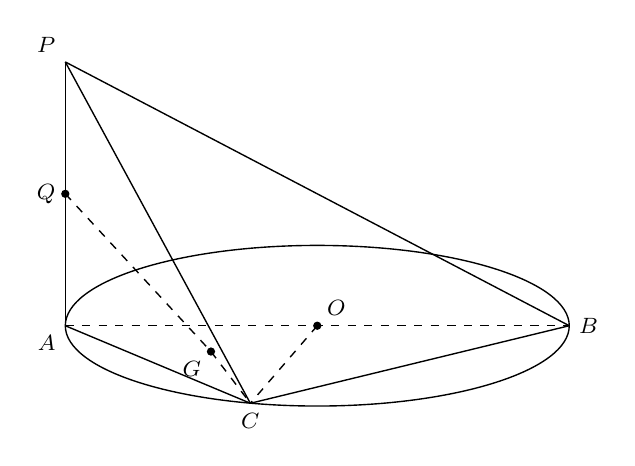
\begin{tikzpicture}[font=\footnotesize, line width=0.5pt, scale=1]
  \coordinate (O) at (0,0);
  \coordinate (A) at (-3.2,0);
  \coordinate (B) at (3.2,0);
  \coordinate (C) at (-0.85,-0.985);
  \coordinate (P) at (-3.2,3.35);
  \coordinate (Q) at (-3.2,1.675);
  \coordinate (G) at (-1.35,-0.328);
  % 底面圆（斜二测画法下的椭圆）
  \draw (0,0) ellipse (3.2 and 1.02);
  % 可见棱
  \draw (P) -- (A);
  \draw (P) -- (B);
  \draw (P) -- (C);
  \draw (A) -- (C);
  \draw (C) -- (B);
  % 被遮挡的线
  \draw[dashed] (A) -- (B);
  \draw[dashed] (O) -- (C);
  \draw[dashed] (Q) -- (G);
  \draw[dashed] (G) -- (C);
  % 点与标签
  \fill (O) circle (1.5pt) node[above right] {$O$};
  \fill (Q) circle (1.5pt) node[left] {$Q$};
  \fill (G) circle (1.5pt) node[below left] {$G$};
  \node[above left] at (P) {$P$};
  \node[below left] at (A) {$A$};
  \node[right] at (B) {$B$};
  \node[below] at (C) {$C$};
\end{tikzpicture}
\end{center}
\nopagebreak[4]
\end{question}
\begin{question}
\gkti{19}现有 $6$ 道题，其中 $4$ 道甲类题，$2$ 道乙类题，张同学从中任取 $2$ 道题解答。试求：

（1） 所取的 $2$ 道题都是甲类题的概率；

（2） 所取的 $2$ 道题不是同一类题的概率。

\Needspace{0.4\textheight}
\end{question}
\begin{question}
\gkti{20}如图，抛物线 $C_1:x^2=4y$，$C_2:x^2=-2py\ (p>0)$。点 $M(x_0,y_0)$ 在抛物线 $C_2$ 上，过 $M$ 作 $C_1$ 的切线，切点为 $A$，$B$（$M$ 为原点 $O$ 时，$A$，$B$ 重合于 $O$）。当 $x_0=1-\sqrt2$ 时，切线 $MA$ 的斜率为 $-\dfrac12$。

（1） 求 $p$ 的值；

（2） 当 $M$ 在 $C_2$ 上运动时，求线段 $AB$ 中点 $N$ 的轨迹方程（$A$，$B$ 重合于 $O$ 时，中点为 $O$）。
\nopagebreak[4]
\begin{center}% 2013 辽宁卷文科第 20 题：抛物线 C1、C2 与过 M 的两条切线。
\begin{tikzpicture}[font=\footnotesize, line width=0.5pt, >=Stealth, scale=1.15]
  % 坐标轴
  \draw[->] (-3.3,0) -- (3.5,0) node[below] {$x$};
  \draw[->] (0,-2.8) -- (0,2.9) node[right] {$y$};
  \node[below right] at (0,0) {$O$};
  % C1: x^2=4y, 即 y=x^2/4
  \draw[domain=-3.15:3.15, smooth, samples=120] plot (\x,{\x*\x/4});
  % C2: x^2=-4y, 即 y=-x^2/4
  \draw[domain=-3.15:3.15, smooth, samples=120] plot (\x,{-\x*\x/4});
  % M(-1,-0.25) 在 C2 上；两条切线的切点
  \coordinate (M) at (-1,-0.25);
  \coordinate (A) at (-2.4142,1.4572);
  \coordinate (B) at (0.4142,0.0429);
  \draw ($(M)!-0.25!(A)$) -- ($(M)!1.22!(A)$);
  \draw ($(M)!-0.25!(B)$) -- ($(M)!1.55!(B)$);
  \fill (M) circle (1.4pt) node[below right] {$M$};
  \node[above] at (A) {$A$};
  \node[above right] at (B) {$B$};
\end{tikzpicture}
\end{center}
\nopagebreak[4]
\end{question}
\begin{question}
\gkti{21}

（1） 证明：当 $x\in[0,1]$ 时，$\dfrac{\sqrt2}2x\leqslant\sin x\leqslant x$；

（2） 若不等式 $ax+x^2+\dfrac{x^3}2+2(x+2)\cos x\leqslant4$ 对 $x\in[0,1]$ 恒成立，求实数 $a$ 的取值范围。

\Needspace{0.4\textheight}
\end{question}
\begin{question}
\gkti{22}如图，$AB$ 为 $\odot O$ 直径，直线 $CD$ 与 $\odot O$ 相切于 $E$，$AD$ 垂直 $CD$ 于 $D$，$BC$ 垂直 $CD$ 于 $C$，$EF$ 垂直 $AB$ 于 $F$，连接 $AE$，$BE$。证明：

（1） $\angle FEB=\angle CEB$；

（2） $EF^2=AD\cdot BC$。
\nopagebreak[4]
\begin{center}% 2013 辽宁卷文科第 22 题：AB 为 ⊙O 直径，CD 切 ⊙O 于 E，AD⊥CD，BC⊥CD，EF⊥AB。
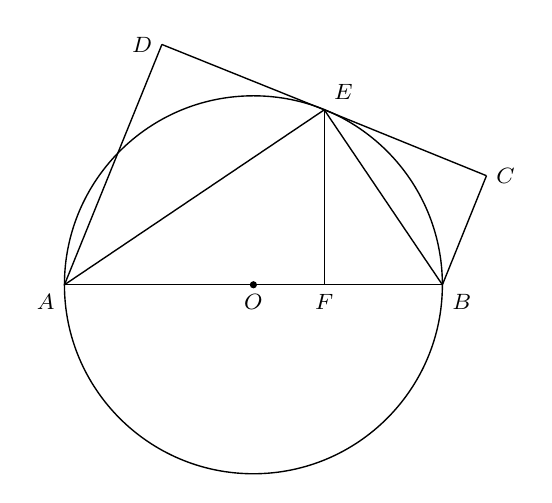
\begin{tikzpicture}[font=\footnotesize, line width=0.5pt, scale=1.0]
  \coordinate (O) at (0,0);
  \coordinate (A) at (-2.4,0);
  \coordinate (B) at (2.4,0);
  \coordinate (E) at (0.90,2.222);
  \coordinate (F) at (0.90,0);
  \coordinate (D) at (-1.162,3.052);
  \coordinate (C) at (2.960,1.385);
  % 圆
  \draw (O) circle (2.4);
  % 直径与切线
  \draw (A) -- (B);
  \draw (D) -- (E) -- (C);
  % 垂线
  \draw (A) -- (D);
  \draw (B) -- (C);
  \draw (E) -- (F);
  % 连接 AE、BE
  \draw (A) -- (E);
  \draw (B) -- (E);
  % 点与标签
  \fill (O) circle (1.3pt) node[below] {$O$};
  \node[below left] at (A) {$A$};
  \node[below right] at (B) {$B$};
  \node[above right] at (E) {$E$};
  \node[left] at (D) {$D$};
  \node[right] at (C) {$C$};
  \node[below] at (F) {$F$};
\end{tikzpicture}
\end{center}
\nopagebreak[4]
\end{question}
\begin{question}
\gkti{23}在直角坐标系 $xOy$ 中，以 $O$ 为极点，$x$ 轴正半轴为极轴建立极坐标系。圆 $C_1$、直线 $C_2$ 的极坐标方程分别为 $\rho=4\sin\theta$，$\rho\cos\left(\theta-\dfrac\pi4\right)=2\sqrt2$。

（1） 求 $C_1$ 与 $C_2$ 交点的极坐标；

\Needspace{5\baselineskip}
（2） 设 $P$ 为 $C_1$ 的圆心，$Q$ 为 $C_1$ 与 $C_2$ 交点连线的中点，已知直线 $PQ$ 的参数方程为
\nopagebreak[4]
\[\begin{cases}x=t^3+a,\\[2pt] y=\dfrac b2t^3+1,\end{cases}\quad (t\in\mathbf R\ \text{\text{为参数}})\]
求 $a$，$b$ 的值。

\end{question}
\begin{question}
\gkti{24}已知函数 $f(x)=|x-a|$，其中 $a>1$。

（1） 当 $a=2$ 时，求不等式 $f(x)\geqslant4-|x-4|$ 的解集；

（2） 已知关于 $x$ 的不等式 $|f(2x+a)-2f(x)|\leqslant2$ 的解集为 $\{x\mid 1\leqslant x\leqslant2\}$，求 $a$ 的值。

\end{question}